% !TEX root = ../../../main.tex
% 来源：中学数学实验教材·第三册（高中数学）
% 章节：函数及其图象 / 函数及其图象
% 原始文件：4.tex，行 1147-1159
% 类型：tikz
% ---
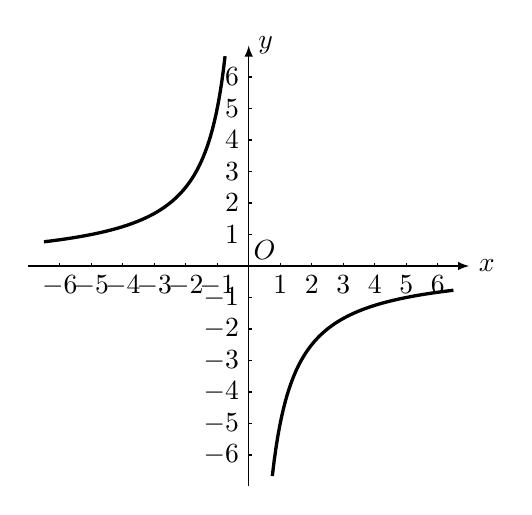
\begin{tikzpicture}[>=latex,scale=.4]
\draw[->] (-7,0)--(7,0)node[right]{$x$};
\draw[->] (0,-7)--(0,7)node[right]{$y$};
\foreach \x in {-6,-5,...,-1,1,2,...,6}
{
    \draw (\x,0)node[below]{$\x$}--(\x,.1);
    \draw (0,\x)node[left]{$\x$}--(.1,\x);
}
\draw [domain=-6.5:-.75, samples=100, very thick] plot(\x, {-5/\x});
\draw [domain=.75:6.5, samples=100, very thick] plot(\x, {-5/\x});
\node at (.5,.5){$O$};

\end{tikzpicture}
